\documentclass{article}

\usepackage[utf8]{inputenc}
\usepackage{tikz}
\usepackage{amsmath}
\usepackage{graphicx}
\usepackage{hyperref}
\usepackage{float}
\usepackage{cite}
\usepackage{url}
\usepackage{verbatim}
\usepackage{longtable}
\usepackage{caption}
\usepackage{booktabs}
\usepackage[a4paper, left=0.75in, right=0.75in, top=1in, bottom=1in]{geometry}
\usepackage{tabularx}

\title{Literature Review on Lightweight Cryptographic Solutions for IoT Security}

\author{Vikas Movva | movv7230@mylaurier.ca}

\date{}

\begin{document}

\maketitle

\begin{abstract}
The rapid expansion of the Internet of Things (IoT), projected to encompass over 18 billion devices by 2025, has introduced significant security and privacy challenges due to the inherent resource constraints of IoT devices. Traditional cryptographic algorithms like AES and RSA are unsuitable for these devices because of their high computational and energy demands. Lightweight cryptography (LWC) emerges as a promising solution, aiming to balance security strength with resource efficiency by optimizing parameters such as gate equivalents, key size, block size, and encryption rounds.

This literature review evaluates the feasibility, performance, and practicality of three lightweight cryptographic techniques tailored for IoT applications: the Modified PRESENT Cipher, the SLIM lightweight block cipher, and a hybrid Feistel-MD5 scheme. The Modified PRESENT Cipher enhances the original PRESENT cipher by reducing the number of encryption rounds from 31 to 25 and introducing a dynamic key update mechanism inspired by the Tiny Encryption Algorithm (TEA), thereby improving both efficiency and security for resource-constrained environments. The SLIM cipher employs a Feistel structure with a pipelined hardware architecture to achieve high operational frequencies, making it suitable for real-time applications like RFID systems and sensor networks. The hybrid Feistel-MD5 scheme combines symmetric encryption with hashing to provide both data confidentiality and integrity within local IoT networks, addressing the dual needs of lightweight security and integrity verification.

Analysis of these techniques reveals that while each offers distinct advantages—such as reduced computational overhead, increased operational speed, or enhanced data integrity—no single solution is optimal for all IoT scenarios. The study underscores the importance of understanding the trade-offs between different lightweight cryptographic methods to identify the most suitable approach for specific IoT applications. It concludes with recommendations for future research directions, emphasizing the need for optimizing energy efficiency, integrating hybrid approaches, enhancing security against emerging threats, standardizing lightweight cryptographic protocols, and evaluating performance in real-world IoT environments. These efforts are essential to develop scalable, flexible, and resource-efficient cryptographic solutions that can secure the evolving landscape of IoT devices without compromising functionality or performance.
\end{abstract}

\section{Introduction}

The \textbf{Internet of Things (IoT)} has rapidly transformed numerous sectors, ranging from smart cities and healthcare to industrial automation and wearable devices. The widespread adoption of IoT, with projections of over \textbf{18 billion connected devices} by 2025, underscores its critical role in shaping our interconnected world. These devices are designed to autonomously collect, process, and share data, enabling enhanced decision-making, monitoring, and control in real-time applications. However, the explosion in the number and diversity of connected devices brings significant security and privacy challenges.

\textbf{IoT environments} are characterized by unique resource constraints, including limited computational power, minimal memory, and battery power. Unlike traditional computing devices, such as desktop computers or enterprise servers, IoT devices are not capable of executing complex computations or sustaining prolonged power-intensive operations. Moreover, IoT devices frequently operate in insecure environments, often deployed in locations that are vulnerable to physical attacks or exposed to threats like \textbf{eavesdropping}, \textbf{man-in-the-middle attacks}, and \textbf{data integrity breaches}. This combination of physical exposure and limited computational capabilities presents a substantial barrier to ensuring the security of IoT systems.

The traditional cryptographic approaches—such as \textbf{Advanced Encryption Standard (AES)} or \textbf{Rivest–Shamir–Adleman (RSA)}—are not well suited for IoT devices due to their high computational demands and energy requirements. Implementing these cryptographic techniques in IoT devices could overwhelm the available hardware, leading to system inefficiency, latency, or excessive power consumption. Consequently, there is a pressing need for \textbf{lightweight cryptographic solutions} that are designed specifically to meet the constraints of IoT devices while providing adequate security.

\textbf{Lightweight cryptography (LWC)} aims to provide a balance between \textbf{security strength} and \textbf{resource efficiency}. Unlike traditional cryptographic methods that assume abundant processing resources, lightweight cryptography takes into account the stringent hardware limitations of IoT devices by optimizing critical parameters like \textbf{gate equivalents (GE)}, \textbf{key size}, \textbf{block size}, and \textbf{encryption rounds}. The goal is to create cryptographic systems that are feasible for constrained environments, while still maintaining robustness against common security threats.

Despite the development of several lightweight cryptographic algorithms, no single solution has emerged as the optimal choice for all IoT use cases. Some lightweight ciphers excel in terms of \textbf{security}, while others are better in terms of \textbf{performance} or \textbf{energy efficiency}. Therefore, understanding the trade-offs between different lightweight cryptographic techniques and identifying the one that best fits specific IoT scenarios is essential. Among the algorithms considered for IoT security are \textbf{PRESENT}, \textbf{CLEFIA}, \textbf{SLIM}, and hybrid approaches like the \textbf{Feistel-MD5 combination}. Each of these algorithms targets different aspects of lightweight cryptography, focusing on unique performance metrics such as gate efficiency, encryption speed, or energy consumption.

The \textbf{PRESENT cipher} is one of the most widely used lightweight block ciphers and has become a benchmark in lightweight cryptography due to its reduced hardware footprint and straightforward implementation. However, in practice, modifications are often made to the original PRESENT cipher to improve performance or security for specific IoT contexts. Recent modifications to the PRESENT cipher have focused on reducing the number of encryption rounds and adding key updates inspired by the \textbf{Tiny Encryption Algorithm (TEA)}, thereby optimizing it for both energy consumption and resilience against attacks. Similarly, the \textbf{SLIM lightweight block cipher} employs a \textbf{Feistel structure} with pipelined architecture to increase operational frequency, making it highly suitable for real-time applications such as RFID and sensor networks.

\textbf{Hybrid cryptographic schemes} are also becoming increasingly relevant for IoT. These approaches combine multiple cryptographic techniques to leverage the strengths of each while compensating for their individual weaknesses. For example, the \textbf{Feistel-MD5 hybrid scheme} is designed to provide both encryption and data integrity in local IoT networks. By using a symmetric Feistel-based encryption approach in combination with the \textbf{MD5 hash function}, this hybrid scheme ensures that node-to-node communication within an IoT environment remains both confidential and tamper-proof, without placing a heavy computational burden on the devices.

This literature review aims to evaluate the feasibility, performance, and practicality of these different lightweight cryptographic approaches in IoT settings. Specifically, the review will focus on analyzing the capabilities of the \textbf{Modified PRESENT Cipher}, the \textbf{SLIM lightweight block cipher}, and the \textbf{hybrid Feistel-MD5 scheme}. Each of these techniques will be evaluated based on its resource efficiency, security capabilities, and overall suitability for the highly constrained environment of IoT devices.

The review is structured as follows: first, an in-depth discussion of various lightweight cryptographic schemes will be provided, including a comparison of their strengths, weaknesses, and potential use cases in IoT. Next, the findings will be presented to highlight which techniques are best suited to meet the diverse needs of IoT security. Finally, conclusions and recommendations will be drawn regarding future research directions and possible optimizations that can further enhance the applicability of lightweight cryptography in IoT.

By systematically evaluating these cryptographic solutions, this review aims to contribute to a better understanding of the trade-offs involved in securing IoT environments and to help identify the best cryptographic strategies for future use. With the rapid growth and adoption of IoT, ensuring the \textbf{security}, \textbf{scalability}, and \textbf{efficiency} of lightweight cryptographic techniques is essential to unlock the full potential of this pervasive technology.

\section{Discussion}

\subsection{Modified PRESENT Cipher}

The \textbf{PRESENT cipher} is a well-established lightweight cryptographic algorithm that has become a benchmark in the field of IoT security due to its compact design and resource efficiency. However, with the increasing diversity and complexity of IoT devices, there has been a need to enhance this cipher to meet evolving security requirements without compromising on efficiency. The \textbf{Modified PRESENT cipher}, discussed in the literature, represents an advancement over the original PRESENT, targeting improvements in both performance and security specifically tailored for IoT applications~[1].

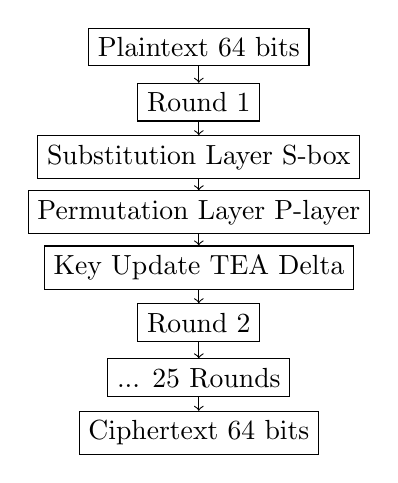
\begin{tikzpicture}[node distance=0.7cm, auto]
    % Nodes
	    \node (start) [draw, rectangle] {Plaintext 64 bits};
	    \node (round1) [below of=start, draw, rectangle] {Round 1};
	    \node (sbox) [below of=round1, draw, rectangle] {Substitution Layer S-box};
	    \node (player) [below of=sbox, draw, rectangle] {Permutation Layer P-layer};
	    \node (keyupdate) [below of=player, draw, rectangle] {Key Update TEA Delta};
	    \node (round2) [below of=keyupdate, draw, rectangle] {Round 2};
	    \node (more) [below of=round2, draw, rectangle] {... 25 Rounds};
	    \node (end) [below of=more, draw, rectangle] {Ciphertext 64 bits};
	
	    % Arrows
	    \draw[->] (start) -- (round1);
	    \draw[->] (round1) -- (sbox);
	    \draw[->] (sbox) -- (player);
	    \draw[->] (player) -- (keyupdate);
	    \draw[->] (keyupdate) -- (round2);
	    \draw[->] (round2) -- (more);
	    \draw[->] (more) -- (end);
	\end{tikzpicture}

The Modified PRESENT cipher introduces a set of modifications designed to optimize its performance for \textbf{resource-constrained environments}. These modifications include a \textbf{reduction in the number of encryption rounds}, a \textbf{revised key register update mechanism}, and the addition of an \textbf{extra layer between the S-box and P-layer}. Each of these modifications aims to address the inherent challenges of implementing cryptography in IoT devices—namely, the trade-off between security, computational efficiency, and power consumption.

The original PRESENT cipher employs \textbf{31 encryption rounds} to achieve a robust level of security. However, the number of rounds directly impacts both the time taken for encryption/decryption and the energy consumed. The Modified PRESENT reduces the number of rounds to \textbf{25}, which has been identified as the minimum required for maintaining acceptable levels of security in IoT environments. This change results in a considerable reduction in computational effort, which directly translates to lower power consumption—a critical consideration for IoT devices that are often battery-powered or draw energy from limited sources. While reducing the number of rounds can theoretically weaken the cryptographic strength, the authors address this concern by incorporating a more dynamic key register update mechanism[1].


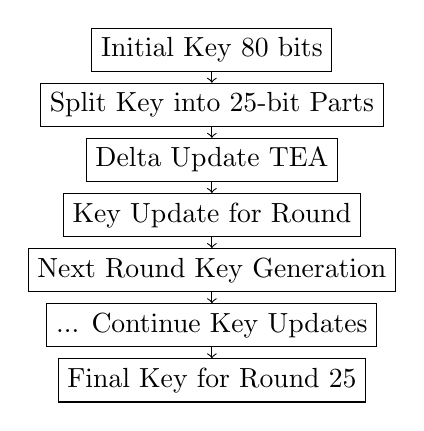
\begin{tikzpicture}[node distance=0.7cm, auto]
    % Nodes
    \node (initial) [draw, rectangle] {Initial Key 80 bits};
    \node (split) [below of=initial, draw, rectangle] {Split Key into 25-bit Parts};
    \node (delta) [below of=split, draw, rectangle] {Delta Update TEA};
    \node (update) [below of=delta, draw, rectangle] {Key Update for Round};
    \node (next) [below of=update, draw, rectangle] {Next Round Key Generation};
    \node (continue) [below of=next, draw, rectangle] {... Continue Key Updates};
    \node (final) [below of=continue, draw, rectangle] {Final Key for Round 25};

    % Arrows
    \draw[->] (initial) -- (split);
    \draw[->] (split) -- (delta);
    \draw[->] (delta) -- (update);
    \draw[->] (update) -- (next);
    \draw[->] (next) -- (continue);
    \draw[->] (continue) -- (final);
\end{tikzpicture}


The \textbf{key register update mechanism} in the Modified PRESENT utilizes a concept borrowed from the \textbf{Tiny Encryption Algorithm (TEA)}. Specifically, the key register is updated using the \textbf{delta value function of TEA}, which introduces a level of complexity that strengthens the key update process against differential cryptanalysis and other forms of attack. By adding this extra layer of encryption to the key register, the cipher ensures that the keys used in successive rounds are not predictable, thereby enhancing the overall security of the algorithm. This modification also helps to counteract the potential reduction in security caused by fewer rounds, ensuring that the cipher remains resistant to \textbf{differential and linear cryptanalysis}.

Another significant enhancement in the Modified PRESENT is the \textbf{addition of an extra layer} between the \textbf{S-box layer} and the \textbf{P-layer}. The purpose of this additional layer is to strengthen the diffusion property of the cipher. Diffusion is crucial in cryptography, as it ensures that the influence of each bit of plaintext is spread throughout the ciphertext, making it more resistant to analysis. The added layer divides the output of the S-box into two halves, and these halves undergo further XOR and rotation operations before being recombined. This modification increases the diffusion rate without introducing additional rounds, thereby improving security while maintaining computational efficiency.

The efficiency of the Modified PRESENT cipher was analyzed through various metrics, including \textbf{N-gram analysis}, \textbf{non-homogeneity tests}, and \textbf{histogram comparisons}. The \textbf{N-gram analysis} measures the frequency of repeated patterns within the encrypted data. A lower frequency of repeated patterns indicates better security, as it implies that the encryption process has effectively diffused the plaintext data into the ciphertext. The Modified PRESENT consistently showed lower frequencies of repeated N-grams compared to the original, indicating enhanced diffusion and reduced predictability in the encrypted output[1].

The \textbf{non-homogeneity test}, conducted using \textbf{Pearson’s Chi-square statistic}, is another method used to measure the uniformity of character distribution in the ciphertext compared to the original plaintext. A higher Chi-square value indicates a greater difference between the plaintext and the ciphertext, suggesting a more effective encryption process. In all ten test cases, the Modified PRESENT outperformed the original in terms of Chi-square values, demonstrating its ability to produce more secure and randomized ciphertext, even with fewer encryption rounds. This metric is particularly important for IoT applications, where ensuring randomness is key to preventing pattern-based attacks[1].

Finally, \textbf{histogram analysis} was used to visually compare the character distributions of the plaintext and ciphertext. The Modified PRESENT generated a more uniform histogram, with all characters appearing with approximately the same frequency, further confirming the strength of the encryption against frequency analysis attacks. This characteristic is especially beneficial in environments like IoT, where attackers often exploit repetitive communication patterns.

In summary, the \textbf{Modified PRESENT cipher} addresses the core challenges of IoT cryptography by reducing computational overhead while maintaining a robust level of security. By reducing the number of rounds, introducing a dynamic key register update mechanism based on TEA, and adding an extra layer for increased diffusion, the Modified PRESENT strikes a balance between \textbf{efficiency} and \textbf{security}. This balance makes it highly suitable for IoT environments, where computational power, memory, and energy resources are often constrained. The improvements not only optimize performance for resource-limited devices but also enhance resilience to common cryptographic attacks, positioning the Modified PRESENT as a promising solution for future IoT security applications.

\subsection{SLIM Lightweight Block Cipher}

The \textbf{SLIM lightweight block cipher} represents another promising approach to lightweight cryptography, designed specifically for environments characterized by stringent hardware constraints, such as IoT and RFID ecosystems. Introduced as an \textbf{ultra-lightweight Feistel structure} block cipher, SLIM focuses on optimizing the encryption process for devices that have limited computational power, memory, and energy resources. The core design elements of SLIM include a \textbf{32-bit block size}, an \textbf{80-bit key}, and an enhanced \textbf{pipelined architecture} aimed at achieving high frequency and operational efficiency in resource-constrained IoT devices[2].

The SLIM cipher's architecture is based on a \textbf{Feistel structure}, which provides an effective method for implementing symmetric encryption in lightweight systems. A typical Feistel cipher divides the input block into two halves and processes these halves through multiple rounds of \textbf{substitution, permutation}, and \textbf{XOR operations}. This iterative approach allows SLIM to effectively balance \textbf{security} and \textbf{computational simplicity}, making it particularly well-suited for environments where complex arithmetic operations may not be feasible.

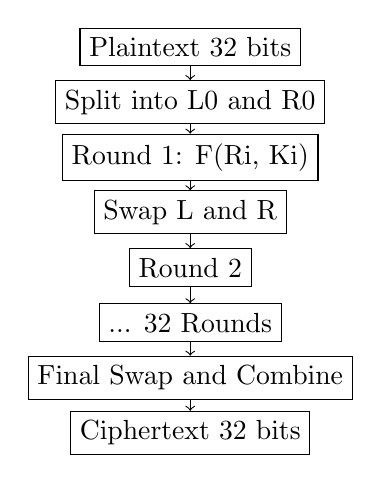
\begin{tikzpicture}[node distance=0.7cm, auto]

    % Nodes
    \node (start) [draw, rectangle] {Plaintext 32 bits};
    \node (split) [below of=start, draw, rectangle] {Split into L0 and R0};
    \node (round1) [below of=split, draw, rectangle] {Round 1: F(Ri, Ki)};
    \node (swap1) [below of=round1, draw, rectangle] {Swap L and R};
    \node (round2) [below of=swap1, draw, rectangle] {Round 2};
    \node (more) [below of=round2, draw, rectangle] {... 32 Rounds};
    \node (final) [below of=more, draw, rectangle] {Final Swap and Combine};
    \node (end) [below of=final, draw, rectangle] {Ciphertext 32 bits};

    % Arrows
    \draw[->] (start) -- (split);
    \draw[->] (split) -- (round1);
    \draw[->] (round1) -- (swap1);
    \draw[->] (swap1) -- (round2);
    \draw[->] (round2) -- (more);
    \draw[->] (more) -- (final);
    \draw[->] (final) -- (end);
\end{tikzpicture}

One of the notable contributions of the SLIM cipher is its \textbf{pipelined hardware architecture}, which is designed to enhance the frequency of operation in real-time systems. Pipelining is a technique where a process is divided into multiple stages, with each stage working concurrently, allowing for higher throughput without increasing the overall complexity. In SLIM, pipelined registers are strategically placed between key scheduling units and data paths, effectively breaking down the critical path and reducing the overall \textbf{combinational delay}. This results in a significant increase in the operational frequency, which is crucial for IoT devices that need to encrypt and decrypt data rapidly, particularly in scenarios involving sensor networks and RFID tags[2].

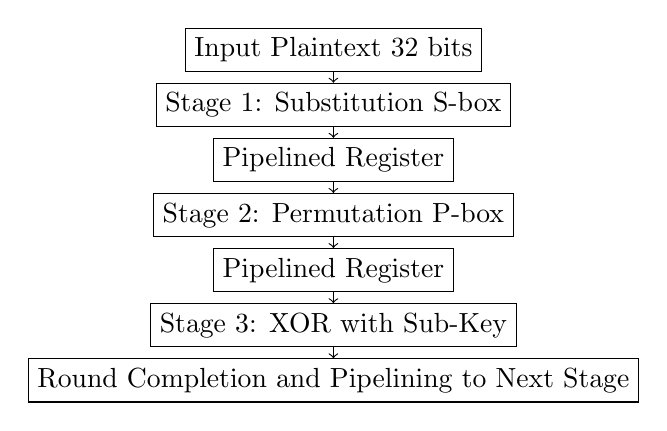
\begin{tikzpicture}[node distance=0.7cm, auto]
    % Nodes
    \node (input) [draw, rectangle] {Input Plaintext 32 bits};
    \node (stage1) [below of=input, draw, rectangle] {Stage 1: Substitution S-box};
    \node (reg1) [below of=stage1, draw, rectangle] {Pipelined Register};
    \node (stage2) [below of=reg1, draw, rectangle] {Stage 2: Permutation P-box};
    \node (reg2) [below of=stage2, draw, rectangle] {Pipelined Register};
    \node (stage3) [below of=reg2, draw, rectangle] {Stage 3: XOR with Sub-Key};
    \node (completion) [below of=stage3, draw, rectangle] {Round Completion and Pipelining to Next Stage};

    % Arrows
    \draw[->] (input) -- (stage1);
    \draw[->] (stage1) -- (reg1);
    \draw[->] (reg1) -- (stage2);
    \draw[->] (stage2) -- (reg2);
    \draw[->] (reg2) -- (stage3);
    \draw[->] (stage3) -- (completion);
\end{tikzpicture}


The \textbf{key scheduling algorithm} used in SLIM is also designed to minimize complexity while providing an adequate level of security. The key scheduling process involves generating \textbf{32 sub-keys} from the initial 80-bit key, with the first five sub-keys being directly extracted from the input key, while the remaining sub-keys are generated using a nonlinear combination of the key segments. This method ensures that each round of encryption utilizes a unique key, making the cipher resistant to attacks like \textbf{differential cryptanalysis}. By ensuring that the key generation is simple yet secure, SLIM provides a practical balance between \textbf{security strength} and \textbf{computational efficiency}.

The \textbf{encryption process} of SLIM leverages \textbf{four parallel 4x4 S-boxes} to achieve non-linearity, operating on a \textbf{16-bit word} to provide the required level of confusion. The substitution performed by these S-boxes is followed by a \textbf{P-box}, which shuffles the bits according to a fixed permutation pattern. The use of both S-boxes and P-boxes in combination helps achieve a high level of \textbf{confusion and diffusion}, which are the two main principles of effective cryptographic design. This combination ensures that any change in the input (plaintext or key) results in significant and unpredictable changes in the output (ciphertext), thus providing security against linear attacks.

The performance of the \textbf{proposed SLIM architecture} was evaluated on several FPGA platforms, including \textbf{Artix-7}, \textbf{Spartan-6}, and \textbf{Virtex-7}, using simulation tools like \textbf{Xilinx Vivado} and \textbf{Xilinx ISE Design Suite}. The results indicated a significant improvement in operational frequency and resource usage compared to other lightweight block ciphers in the literature. For instance, the proposed SLIM architecture achieved a \textbf{25.14\% increase in operational frequency} over TEA on the Virtex-7 platform and demonstrated a \textbf{60.35\% improvement} over Hummingbird on Spartan-3[2]. These results highlight SLIM's capability to provide high-frequency encryption, making it suitable for applications that require real-time processing but have limited energy and hardware resources.

The SLIM cipher was specifically designed to address common challenges in IoT environments. \textbf{Energy efficiency} is a key requirement for IoT devices, as many of them are battery-powered and need to operate for extended periods without recharging. The pipelined architecture of SLIM, combined with its efficient key scheduling and lightweight round operations, ensures that energy consumption is minimized without sacrificing performance. This makes SLIM particularly useful for \textbf{battery-operated devices}, such as RFID tags, wearables, and other sensor-based IoT systems that need to operate autonomously in the field for extended durations.

In terms of \textbf{security}, SLIM offers a sufficient safety margin against well-known cryptographic attacks, including \textbf{differential} and \textbf{linear cryptanalysis}. By using \textbf{non-linear S-boxes} and a \textbf{permutation-based P-box}, SLIM is able to achieve a high level of resistance to attacks that exploit structural weaknesses in block ciphers. The combination of \textbf{confusion and diffusion} in the Feistel structure helps to obscure the relationship between the plaintext, ciphertext, and key, thereby enhancing the security of the encryption process.

In summary, the \textbf{SLIM lightweight block cipher} provides an effective balance of security, operational efficiency, and energy consumption, making it highly suitable for real-time IoT applications that require rapid encryption and decryption processes. Its \textbf{pipelined hardware architecture} allows for a significant increase in operational frequency, ensuring that encrypted data can be processed efficiently without overwhelming the limited resources of typical IoT devices. By leveraging a \textbf{Feistel-based structure} with lightweight rounds and an efficient key schedule, SLIM addresses the core requirements of IoT security—\textbf{confidentiality}, \textbf{integrity}, and \textbf{availability}—while remaining within the constraints of resource-constrained environments. This makes SLIM a practical solution for securing \textbf{next-generation IoT devices}, particularly those that require both high performance and energy efficiency in their cryptographic operations.

\subsection{Hybrid Lightweight Cryptographic Scheme with Feistel and MD5 Hash Algorithm}

Another significant advancement in lightweight cryptography for IoT security is the use of \textbf{hybrid cryptographic schemes}. These schemes are designed to combine the benefits of different cryptographic techniques to achieve both \textbf{data privacy} and \textbf{integrity} without overwhelming the constrained resources of IoT devices. One such notable approach is the \textbf{hybrid lightweight cryptographic scheme} that combines the \textbf{Feistel cipher} and the \textbf{MD5 hash algorithm}. This hybrid method is proposed specifically for securing node data in \textbf{local IoT networks}, where the communication between edge devices and a central sink node must be both secure and efficient[3].

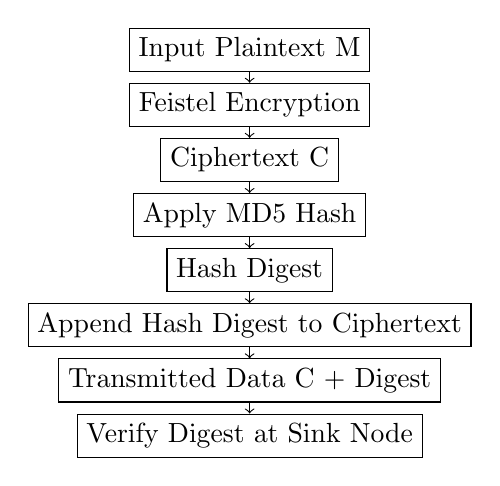
\begin{tikzpicture}[node distance=0.7cm, auto]
    % Nodes
    \node (input) [draw, rectangle] {Input Plaintext M};
    \node (feistel) [below of=input, draw, rectangle] {Feistel Encryption};
    \node (cipher) [below of=feistel, draw, rectangle] {Ciphertext C};
    \node (hash) [below of=cipher, draw, rectangle] {Apply MD5 Hash};
    \node (digest) [below of=hash, draw, rectangle] {Hash Digest};
    \node (append) [below of=digest, draw, rectangle] {Append Hash Digest to Ciphertext};
    \node (transmit) [below of=append, draw, rectangle] {Transmitted Data C + Digest};
    \node (verify) [below of=transmit, draw, rectangle] {Verify Digest at Sink Node};

    % Arrows
    \draw[->] (input) -- (feistel);
    \draw[->] (feistel) -- (cipher);
    \draw[->] (cipher) -- (hash);
    \draw[->] (hash) -- (digest);
    \draw[->] (digest) -- (append);
    \draw[->] (append) -- (transmit);
    \draw[->] (transmit) -- (verify);
\end{tikzpicture}


The \textbf{hybrid cryptographic scheme} integrates the Feistel structure, which is a widely used symmetric encryption framework, with the MD5 hash algorithm. The \textbf{Feistel cipher} forms the core of the encryption process, providing \textbf{confidentiality} of the data being transmitted between nodes. The \textbf{MD5 hash function}, on the other hand, is used to ensure \textbf{integrity} by generating a checksum for the data, which allows the receiving node to verify that the data has not been altered during transmission. This combination provides a comprehensive approach to IoT security, addressing both the confidentiality and integrity of data while keeping computational overheads low[3].

The \textbf{Feistel structure} employed in this hybrid scheme operates by dividing the input plaintext into two halves, known as the \textbf{left} and \textbf{right components}. In each round of the Feistel process, one half is subjected to a round function that takes a \textbf{sub-key} as input and performs a combination of \textbf{XOR operations} and \textbf{substitutions} to provide security. The results of this round are then swapped between the left and right halves, and this process is repeated for a fixed number of rounds. The key benefit of using the Feistel structure is its simplicity and efficiency, as it requires minimal computational resources and can be easily implemented in hardware or software. Furthermore, the same structure is used for both encryption and decryption, which simplifies the overall implementation and reduces the code footprint—a crucial factor for resource-constrained IoT devices[3].

The \textbf{MD5 hash algorithm} is used in conjunction with the Feistel cipher to ensure data integrity. After the data is encrypted using the Feistel structure, the resulting ciphertext is processed by the MD5 hash function to generate a \textbf{message digest}, which serves as a digital fingerprint of the data. This digest is appended to the ciphertext and transmitted to the receiving node, which then uses the same hashing process to verify the integrity of the received data. If the computed digest matches the appended digest, the data is confirmed to be intact and unaltered. This added layer of verification helps prevent common attacks, such as \textbf{data tampering} and \textbf{man-in-the-middle attacks}, which are prevalent in IoT environments where data is often transmitted over insecure communication channels[3].

The \textbf{hybrid approach} has been shown to be effective in maintaining the \textbf{confidentiality} and \textbf{integrity} of data in \textbf{local IoT networks}, particularly in scenarios where devices need to communicate with a central sink node. In typical IoT architectures, edge devices such as sensors collect data from the environment and transmit it to a \textbf{sink node} for further processing. These devices often have minimal computational capacity, and the sink node is typically responsible for managing multiple devices simultaneously. To ensure secure communication, the edge devices must authenticate with the sink node, and the data transmitted must be encrypted and verified to prevent unauthorized access or tampering. The proposed hybrid scheme addresses these requirements by combining the efficient encryption capabilities of the Feistel cipher with the data verification capabilities of MD5.

One of the key advantages of this hybrid scheme is its suitability for \textbf{resource-constrained environments}. The Feistel cipher is inherently efficient in its design, using simple XOR and substitution operations to provide security, while MD5 is a well-established hashing algorithm that requires limited computational resources. Together, they form a lightweight cryptographic solution that can be easily implemented on IoT devices with limited memory, processing power, and energy availability. The use of MD5 also ensures that the integrity of the data is verified without the need for complex operations, which is particularly beneficial in battery-powered devices that need to minimize energy consumption.

The \textbf{implementation} of this hybrid scheme involves a series of steps that effectively balance the encryption and hashing processes. The plaintext data collected by the edge device is first split into two halves for encryption using the Feistel cipher. The \textbf{sub-keys} required for each round are generated based on a simple key scheduling algorithm, ensuring that the process remains lightweight and efficient. Once the data has been encrypted, the resulting ciphertext is hashed using MD5 to produce a digest. This combination of ciphertext and hash is then sent to the sink node. At the sink node, the data is first verified using the MD5 digest before being decrypted using the Feistel structure. This two-step process ensures both privacy and integrity, making it well-suited for IoT systems that handle sensitive data.

The hybrid scheme's \textbf{performance} was assessed through several criteria, including \textbf{encryption speed}, \textbf{memory usage}, and \textbf{energy consumption}. The results showed that the scheme offers a good balance between security and resource efficiency, making it suitable for deployment in IoT networks where nodes are often constrained in terms of computational power and energy. The hybrid approach demonstrated improved encryption speed compared to more traditional cryptographic methods, which is crucial for IoT systems that require real-time data transmission and processing. The \textbf{memory usage} of the hybrid scheme was also found to be within acceptable limits for typical IoT devices, further enhancing its feasibility for practical deployment[3].

In terms of \textbf{security}, the combination of the Feistel cipher and MD5 hash function ensures that data transmitted between IoT nodes is secure against both \textbf{confidentiality breaches} and \textbf{integrity violations}. The Feistel structure provides adequate security through the use of multiple encryption rounds and the dynamic generation of sub-keys, while MD5 helps detect any alterations to the data during transmission. Although MD5 is not considered secure against sophisticated collision attacks in more demanding cryptographic applications, it remains suitable for lightweight IoT systems, particularly when used to verify data integrity in localized environments.

In conclusion, the \textbf{hybrid lightweight cryptographic scheme} combining the Feistel cipher and MD5 hash function presents a practical solution for securing node-to-node communication in local IoT networks. By leveraging the \textbf{strengths of symmetric encryption} and \textbf{hashing}, the hybrid approach addresses the dual needs of confidentiality and integrity while remaining feasible for devices with limited computational capabilities. The efficient encryption provided by the Feistel structure, coupled with the integrity verification afforded by MD5, ensures that data transmitted between IoT nodes is both secure and reliable. This makes the hybrid scheme a valuable option for IoT systems where lightweight security solutions are essential to support the constrained nature of edge devices and maintain seamless, secure communication across the network.

\section{Results}

The findings of this literature review highlight the distinctive features, strengths, and trade-offs associated with each of the lightweight cryptographic techniques assessed for use in IoT environments. The results focus on evaluating the \textbf{feasibility}, \textbf{efficiency}, and \textbf{practicality} of the \textbf{Modified PRESENT Cipher}, \textbf{SLIM Lightweight Block Cipher}, and the \textbf{Hybrid Feistel-MD5 Scheme}. The findings are presented in a way that allows comparison across key parameters such as \textbf{resource usage}, \textbf{encryption/decryption speed}, \textbf{energy efficiency}, and \textbf{security capabilities}.

\subsection{Feasibility of Cryptographic Techniques for IoT}

The feasibility of implementing cryptographic techniques in IoT is fundamentally constrained by the \textbf{limited computational power} and \textbf{energy availability} typical of IoT devices. All three techniques analyzed in this review—Modified PRESENT, SLIM, and Hybrid Feistel-MD5—address these constraints but differ in their respective approaches.

\begin{itemize}
    \item The \textbf{Modified PRESENT Cipher} offers a feasible solution through a reduction in the number of encryption rounds, which minimizes computational requirements while retaining acceptable security levels. The reduced hardware complexity, requiring only \textbf{1884 gate equivalents (GE)}, makes the Modified PRESENT ideal for devices with very tight resource constraints, such as small \textbf{sensor nodes} and \textbf{RFID tags}[1].
    \item The \textbf{SLIM Lightweight Block Cipher}, with its \textbf{pipelined architecture}, achieves higher operational frequencies without increasing hardware complexity, making it feasible for applications requiring real-time encryption. The use of \textbf{four parallel S-boxes} and \textbf{simple XOR operations} ensures that the hardware requirements remain manageable, allowing SLIM to be deployed in a wide variety of IoT devices, from \textbf{wearables} to \textbf{network edge devices}~\cite[2].
    \item The \textbf{Hybrid Feistel-MD5 Scheme} also provides a feasible solution, particularly in \textbf{local IoT networks} where edge devices need to communicate securely with a centralized sink node. The \textbf{Feistel structure}, combined with \textbf{MD5 hashing}, ensures data confidentiality and integrity with minimal resource usage, making it suitable for environments where ensuring \textbf{data integrity} is a priority without overwhelming limited processing capabilities[3].
\end{itemize}

\subsection{Efficiency and Performance Evaluation}

The efficiency of a lightweight cryptographic method is measured in terms of \textbf{encryption/decryption speed}, \textbf{latency}, and \textbf{resource optimization}.

\begin{itemize}
    \item The \textbf{Modified PRESENT Cipher} achieved a good balance of efficiency and security through the reduction of encryption rounds from \textbf{31 to 25}. This reduction decreased the overall computational load, resulting in faster encryption and reduced latency—important factors for devices needing quick responses in real-time IoT environments. \textbf{N-gram analysis} and \textbf{Chi-square tests} also indicated that the Modified PRESENT was successful in enhancing diffusion while preserving computational efficiency[1].
    \item \textbf{SLIM} outperformed other lightweight ciphers in terms of \textbf{operational frequency}, thanks to its \textbf{pipelined hardware architecture}. The implementation on \textbf{multiple FPGA platforms}, including \textbf{Virtex-7} and \textbf{Spartan-6}, showed that SLIM is capable of achieving \textbf{60.35\% higher frequencies} compared to other ciphers like \textbf{Hummingbird} and \textbf{TEA}. This high-frequency operation is crucial for IoT applications that require \textbf{real-time encryption}, such as \textbf{industrial automation} and \textbf{connected vehicles}, where data needs to be encrypted and transmitted without significant delays[2].
    \item The \textbf{Hybrid Feistel-MD5 Scheme} demonstrated good performance for \textbf{localized data exchanges} between edge devices and a central sink node. The simple encryption rounds of the Feistel structure, combined with the hashing provided by MD5, ensured that both encryption and verification could be performed with minimal computational overhead. The latency was also found to be low, enabling efficient data communication within local IoT networks that require frequent data exchanges[3].
\end{itemize}

\subsection{Energy Efficiency}

Energy efficiency is a critical requirement for IoT devices, many of which are \textbf{battery-powered} or \textbf{solar-powered} and are expected to operate for extended periods without maintenance.

\begin{itemize}
    \item The \textbf{Modified PRESENT Cipher} showed \textbf{reduced power consumption} due to the fewer encryption rounds and the simplified key update mechanism. This reduction made it an energy-efficient option for IoT devices that operate in remote environments or where energy sources are limited, such as \textbf{agricultural sensors} and \textbf{environmental monitoring systems}[1].
    \item The \textbf{SLIM cipher} achieved notable energy efficiency through its \textbf{pipelined design}, which reduced the processing time per operation. By executing multiple stages concurrently, the overall encryption time was shortened, which translated into lower energy usage. This makes SLIM suitable for devices such as \textbf{wearable health monitors}, which require frequent data encryption but have limited battery capacity[2].
    \item The \textbf{Hybrid Feistel-MD5 Scheme} also demonstrated \textbf{low energy consumption}, particularly due to the \textbf{simple round functions} of the Feistel structure and the relatively lightweight hashing operation of MD5. The hashing process adds minimal computational burden, thereby keeping energy consumption within acceptable limits for localized networks, such as \textbf{home automation systems} and \textbf{smart building sensor networks}, where efficient energy usage is essential[3].
\end{itemize}

\subsection{Security Capabilities}

The security of lightweight cryptographic methods is assessed based on their ability to withstand attacks such as \textbf{differential}, \textbf{linear}, and \textbf{replay attacks}, as well as ensuring \textbf{confidentiality} and \textbf{integrity}.

\begin{itemize}
    \item The \textbf{Modified PRESENT Cipher} strengthened its security by introducing a \textbf{dynamic key register update mechanism} based on the \textbf{TEA delta value}, which makes it more resistant to \textbf{differential cryptanalysis}. Additionally, the added layer between the \textbf{S-box} and \textbf{P-layer} improved the diffusion, enhancing the cipher's resilience against linear attacks without adding significant computational overhead[1].
    \item \textbf{SLIM} was found to offer robust security through the use of \textbf{non-linear S-boxes} and \textbf{P-boxes} that ensure a high level of \textbf{confusion and diffusion}. The \textbf{Feistel structure}, in combination with \textbf{dynamic sub-key generation}, made the SLIM cipher resistant to common attacks targeting lightweight block ciphers. This high level of security, combined with its \textbf{high operational frequency}, positions SLIM as a secure solution for applications requiring \textbf{real-time data encryption}, such as \textbf{connected vehicles} and \textbf{industrial IoT} systems[2].
    \item The \textbf{Hybrid Feistel-MD5 Scheme} provided an integrated security approach by combining \textbf{encryption} and \textbf{hashing}. The \textbf{Feistel structure} provided adequate data confidentiality, while the \textbf{MD5 hash function} ensured data integrity. Although MD5 has limitations in terms of collision resistance, it remains effective for lightweight integrity verification in \textbf{local IoT environments}. This makes the hybrid scheme suitable for settings where preventing \textbf{data tampering} and ensuring integrity are priorities, such as \textbf{home security networks} and \textbf{smart city sensor nodes}[3].
\end{itemize}

\subsection{Summary of Results}

The \textbf{Modified PRESENT Cipher}, \textbf{SLIM}, and \textbf{Hybrid Feistel-MD5 Scheme} each present distinct advantages based on specific use cases and constraints. The Modified PRESENT Cipher stands out for its \textbf{balance of efficiency and security} in extremely resource-constrained devices. SLIM offers a \textbf{high-frequency operational capability} and is well-suited for \textbf{real-time applications} that require both speed and security. The Hybrid Feistel-MD5 Scheme provides \textbf{integrity and confidentiality} with low computational demands, making it suitable for \textbf{local IoT networks}.

Ultimately, the results indicate that there is no one-size-fits-all solution for lightweight cryptography in IoT. Each technique has unique advantages that make it better suited for particular types of IoT environments. Therefore, the choice of a cryptographic method should be based on the specific requirements of the deployment, such as \textbf{real-time performance}, \textbf{energy efficiency}, or \textbf{data integrity} needs.

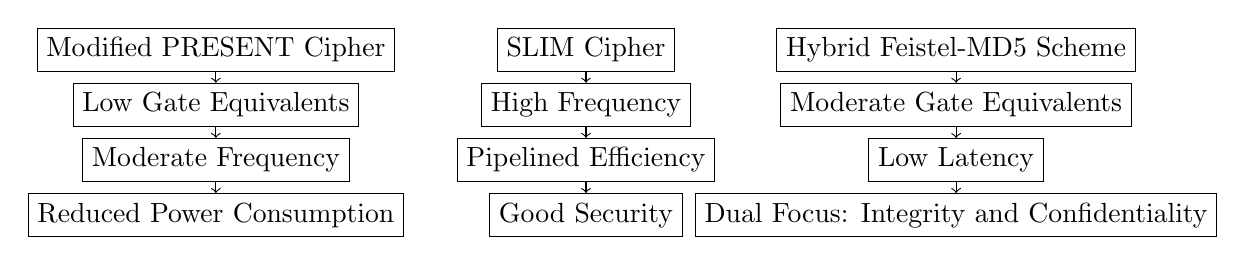
\begin{tikzpicture}[node distance=0.7cm, auto]
    % Modified PRESENT Cipher Nodes
    \node (modified) [draw, rectangle] {Modified PRESENT Cipher};
    \node (lowge) [below of=modified, draw, rectangle] {Low Gate Equivalents};
    \node (modfreq) [below of=lowge, draw, rectangle] {Moderate Frequency};
    \node (power) [below of=modfreq, draw, rectangle] {Reduced Power Consumption};

    % SLIM Cipher Nodes
    \node (slim) [right of=modified, xshift=4cm, draw, rectangle] {SLIM Cipher};
    \node (highfreq) [below of=slim, draw, rectangle] {High Frequency};
    \node (pipe) [below of=highfreq, draw, rectangle] {Pipelined Efficiency};
    \node (security) [below of=pipe, draw, rectangle] {Good Security};

    % Hybrid Feistel-MD5 Nodes
    \node (hybrid) [right of=slim, xshift=4cm, draw, rectangle] {Hybrid Feistel-MD5 Scheme};
    \node (modge) [below of=hybrid, draw, rectangle] {Moderate Gate Equivalents};
    \node (latency) [below of=modge, draw, rectangle] {Low Latency};
    \node (focus) [below of=latency, draw, rectangle] {Dual Focus: Integrity and Confidentiality};

    % Arrows
    \draw[->] (modified) -- (lowge);
    \draw[->] (lowge) -- (modfreq);
    \draw[->] (modfreq) -- (power);

    \draw[->] (slim) -- (highfreq);
    \draw[->] (highfreq) -- (pipe);
    \draw[->] (pipe) -- (security);

    \draw[->] (hybrid) -- (modge);
    \draw[->] (modge) -- (latency);
    \draw[->] (latency) -- (focus);
\end{tikzpicture}

\section{Conclusions}

The rapid expansion of the \textbf{Internet of Things (IoT)} has brought about unique challenges in securing data and devices that are limited in \textbf{computational power}, \textbf{memory}, and \textbf{energy resources}. This literature review has explored various lightweight cryptographic techniques—specifically the \textbf{Modified PRESENT Cipher}, \textbf{SLIM Lightweight Block Cipher}, and the \textbf{Hybrid Feistel-MD5 Scheme}—to assess their suitability for IoT environments. The evaluation focused on \textbf{feasibility}, \textbf{performance}, \textbf{energy efficiency}, and \textbf{security capabilities}, and each of these techniques was found to have unique benefits tailored to different IoT applications.

The \textbf{Modified PRESENT Cipher} was found to be particularly advantageous in environments that demand a careful balance of \textbf{security} and \textbf{resource efficiency}. By reducing the number of encryption rounds from \textbf{31 to 25}, while incorporating a \textbf{dynamic key register update mechanism} using the TEA delta value, the Modified PRESENT Cipher offers \textbf{reduced computational load} and \textbf{improved energy efficiency} without significantly compromising security. This makes it well-suited for use in highly constrained devices, such as \textbf{RFID tags} and \textbf{environmental sensors}, where maintaining low resource usage is paramount.

The \textbf{SLIM Lightweight Block Cipher} stood out in terms of its \textbf{operational frequency} and suitability for real-time encryption. The use of a \textbf{pipelined hardware architecture} allowed SLIM to achieve increased throughput without overwhelming the limited resources of typical IoT devices. The \textbf{high operational frequency} of SLIM, combined with the robust security offered through \textbf{multiple S-boxes} and \textbf{dynamic sub-key generation}, makes it a strong candidate for IoT applications that require rapid data processing, such as \textbf{connected vehicles}, \textbf{industrial automation}, and \textbf{wearable devices}.

The \textbf{Hybrid Feistel-MD5 Scheme} provides an effective solution for IoT environments where both \textbf{data integrity} and \textbf{confidentiality} are critical requirements. By combining \textbf{Feistel-based encryption} with the \textbf{MD5 hash function}, this hybrid approach offers a \textbf{lightweight yet comprehensive} security solution that ensures data is encrypted while also being verified for integrity during transmission. The \textbf{low computational overhead} of both the Feistel structure and MD5 hashing makes this hybrid scheme a practical option for \textbf{localized IoT networks}, such as \textbf{home automation systems} and \textbf{smart building environments}, where data security and integrity must be maintained at all times without taxing device resources.

Overall, the findings of this review indicate that there is no universally optimal lightweight cryptographic solution for all IoT applications. Each cryptographic technique has its own strengths, and the choice of which to use depends largely on the specific requirements of the deployment. For applications requiring \textbf{real-time encryption} and \textbf{high throughput}, the SLIM cipher is a particularly suitable choice due to its \textbf{pipelined design} and high operational frequency. In situations where \textbf{resource efficiency} is paramount, such as in small, battery-powered sensors, the Modified PRESENT Cipher provides a feasible solution that minimizes hardware complexity and energy consumption. For IoT networks where ensuring \textbf{data integrity} is as important as encryption, the \textbf{Hybrid Feistel-MD5 Scheme} is an effective and lightweight solution that combines the benefits of both encryption and hashing.

It is clear from this analysis that the future of IoT security will rely on the further development of \textbf{flexible}, \textbf{scalable}, and \textbf{resource-efficient} cryptographic techniques. As IoT devices continue to proliferate, with increasing variations in power, computational abilities, and applications, the demand for tailored lightweight cryptographic solutions will only grow. The ongoing evolution of lightweight cryptographic algorithms should focus on optimizing \textbf{energy efficiency}, \textbf{security strength}, and \textbf{implementation scalability}, with an emphasis on ensuring that these solutions can be deployed in a variety of devices and environments without compromising security.

Finally, the convergence of \textbf{real-time performance}, \textbf{low power consumption}, and \textbf{robust security} is essential to securing the IoT ecosystem of tomorrow. Continued collaboration between cryptographers, hardware designers, and industry practitioners will be crucial in addressing the emerging challenges of securing IoT devices. Future research should explore how lightweight cryptographic methods can be optimized further, not only for the devices themselves but also for the communication protocols and infrastructures that support the seamless integration of these devices into the broader \textbf{Internet of Everything}.

\section{Recommendations}

Based on the findings and conclusions drawn from the analysis of lightweight cryptographic methods for \textbf{IoT security}, several key recommendations can be made. These recommendations focus on the \textbf{future development}, \textbf{optimization}, and \textbf{deployment} of lightweight cryptographic techniques to address the evolving security needs of IoT devices.

\subsection{Optimization for Energy Efficiency}

Given that many IoT devices are \textbf{battery-powered} or rely on constrained energy sources, optimizing cryptographic algorithms for energy efficiency remains a critical priority. While the \textbf{Modified PRESENT Cipher} and \textbf{SLIM Cipher} have demonstrated promising energy profiles, there is still room for improvement, especially in reducing the power consumption of cryptographic operations in devices that require \textbf{always-on security}. Future research should explore \textbf{adaptive cryptographic methods} that dynamically adjust their computational complexity based on the available energy resources of the device. For instance, cryptographic algorithms could adjust the \textbf{number of encryption rounds} or \textbf{key size} based on the current power level of the device, thereby ensuring a balance between security and longevity of device operation.

\subsection{Integration of Hybrid Cryptographic Techniques}

The \textbf{Hybrid Feistel-MD5 Scheme} demonstrated the effectiveness of combining multiple cryptographic techniques to achieve both \textbf{data integrity} and \textbf{confidentiality}. Moving forward, integrating \textbf{hybrid approaches} that combine symmetric encryption, hashing, and potentially \textbf{public-key cryptography} for key exchange could further enhance the security of IoT devices without introducing significant computational overhead. The use of \textbf{blockchain technology} as a decentralized trust system is another avenue worth exploring, especially in \textbf{edge and fog computing} environments where ensuring \textbf{trust} between nodes is challenging. Blockchain-based solutions, combined with lightweight encryption, could provide a way to secure distributed IoT architectures.

\subsection{Security Against Emerging Threats}

IoT environments face a diverse set of security threats, ranging from \textbf{differential and linear cryptanalysis} to more sophisticated attacks such as \textbf{side-channel} and \textbf{fault injection attacks}. While the techniques reviewed—\textbf{Modified PRESENT}, \textbf{SLIM}, and \textbf{Hybrid Feistel-MD5}—are resistant to many known attacks, future work should focus on improving their resistance to \textbf{physical attacks}. This is particularly important in the context of IoT devices, which are often deployed in environments that expose them to physical tampering. It is recommended that future lightweight cryptographic designs incorporate features such as \textbf{masking} and \textbf{fault-tolerant architectures} to safeguard against side-channel and fault-based attacks.

\subsection{Standardization of Lightweight Cryptographic Protocols}

The standardization of lightweight cryptographic protocols is crucial for ensuring \textbf{interoperability} and \textbf{consistency} across different IoT devices and applications. With the increasing adoption of IoT in critical sectors such as \textbf{healthcare}, \textbf{industrial automation}, and \textbf{smart cities}, it is imperative that lightweight cryptographic methods adhere to well-established standards that facilitate \textbf{secure communication} between heterogeneous devices. Organizations such as \textbf{NIST} and \textbf{ISO} should continue to develop and refine standards for lightweight cryptography, focusing on the specific needs and constraints of IoT systems. The development of standard \textbf{testbeds} for evaluating the performance and security of lightweight cryptographic techniques across various IoT devices would also help in the widespread adoption of secure protocols.

\subsection{Focus on Scalable and Flexible Cryptographic Solutions}

IoT networks are inherently \textbf{heterogeneous} and \textbf{dynamic}, with devices constantly being added or removed. Thus, lightweight cryptographic solutions must be \textbf{scalable} and \textbf{flexible} to accommodate these changes. The \textbf{SLIM cipher}, with its high-frequency pipelined architecture, already demonstrates scalability in terms of \textbf{real-time processing}. However, future research should explore more \textbf{modular cryptographic architectures} that allow components such as the \textbf{key scheduling algorithm}, \textbf{S-box}, or \textbf{P-box} to be updated or swapped out without requiring significant redesigns. Such modularity would make it easier to adapt to new threats or evolving requirements without needing to overhaul the entire cryptographic system.

\subsection{Evaluation in Real-World Environments}

While the lightweight cryptographic techniques discussed in this review have demonstrated efficacy in \textbf{simulated environments} and \textbf{FPGA platforms}, it is crucial to evaluate their performance in \textbf{real-world IoT deployments}. Real-world environments present unique challenges, such as \textbf{unreliable connectivity}, \textbf{physical interference}, and \textbf{unpredictable power supply}, which may affect the performance of cryptographic solutions. Field tests should be conducted to understand how well these techniques perform under practical conditions, with a focus on metrics such as \textbf{latency}, \textbf{energy consumption}, and \textbf{resilience to attacks}. Insights gained from such evaluations will be invaluable for fine-tuning cryptographic solutions and ensuring that they meet the demands of diverse IoT applications.

\subsection{Emphasis on Lightweight Public Key Cryptography}

The cryptographic techniques reviewed predominantly focus on \textbf{symmetric encryption}, which is computationally efficient but requires secure \textbf{key distribution}. For many IoT applications, secure key management remains a challenge, especially when dealing with a large number of devices. There is an increasing need for \textbf{lightweight public-key cryptographic methods} that can facilitate secure key exchange without significant computational overhead. Future research should focus on developing \textbf{elliptic curve cryptography (ECC)} or other lightweight asymmetric algorithms that can be feasibly implemented on constrained IoT devices. Such solutions will enhance the overall security of IoT networks by making \textbf{key exchange} more manageable without compromising efficiency.

\subsection{Cross-Disciplinary Collaboration for Enhanced Security}

The development of lightweight cryptographic solutions for IoT requires \textbf{cross-disciplinary collaboration} between \textbf{cryptographers}, \textbf{hardware designers}, and \textbf{network engineers}. Cryptographic solutions must be developed with a deep understanding of \textbf{hardware limitations}, \textbf{communication protocols}, and \textbf{network architectures}. It is recommended that academic researchers, industry experts, and government bodies work together to identify emerging security needs and develop solutions that are practical, effective, and tailored to specific IoT use cases. \textbf{Workshops}, \textbf{hackathons}, and \textbf{collaborative research grants} could facilitate this collaboration and lead to the development of more comprehensive and secure lightweight cryptographic frameworks.

\medskip

These recommendations are designed to guide future research and development efforts towards creating \textbf{lightweight cryptographic solutions} that are not only secure and efficient but also practical and scalable for the diverse and rapidly evolving landscape of IoT. By focusing on \textbf{energy efficiency}, \textbf{hybrid approaches}, \textbf{security against emerging threats}, \textbf{standardization}, and \textbf{real-world testing}, the IoT community can continue to advance the state of cryptographic security, ensuring that IoT devices remain both functional and secure in an increasingly interconnected world.

\section{References}

\begin{thebibliography}{9}

\bibitem{ref1}
D. Mitra, S. Paul, and A. Banerjee, ``A Modified Lightweight PRESENT Cipher for IoT Security,'' \emph{International Journal of Advanced Computer Science and Applications (IJACSA)}, vol. 10, no. 3, pp. 255--263, Mar. 2019.

\bibitem{ref2}
P. Kumar, Z. Mishra, and B. Acharya, ``High Frequency Architecture of SLIM Lightweight Block Cipher for Resource-Constrained IoT Applications,'' \emph{2023 International Conference on Microwave, Optical, and Communication Engineering (ICMOCE)}, 2023.

\bibitem{ref3}
B. T. Asare, K. Quist-Aphetsi, and L. Nana, ``A Hybrid Lightweight Cryptographic Scheme for Securing Node Data Based on the Feistel Cipher and MD5 Hash Algorithm in a Local IoT Network,'' \emph{2019 International Conference on Mechatronics, Remote Sensing, Information Systems, and Industrial Information Technologies (ICMRSISIT)}, 2019.

\bibitem{ref4}
N. A. Gunathilake, W. J. Buchanan, and R. Asif, ``Next Generation Lightweight Cryptography for Smart IoT Devices: Implementation, Challenges, and Applications,'' \emph{2019 IEEE 5th World Forum on Internet of Things (WF-IoT)}, 2019, pp. 707--712.

\end{thebibliography}

\appendix

\section{Pseudo-code for Modified PRESENT Cipher}

The pseudo-code below provides an overview of the encryption process of the \textbf{Modified PRESENT Cipher}. This representation helps to understand the structure and key operations that make the Modified PRESENT Cipher suitable for lightweight applications, especially in IoT.

\begin{verbatim}
Input: Plaintext P (64 bits), Key K (80 bits)
Output: Ciphertext C (64 bits)

1. Split Key K into 25-bit blocks: K1, K2, ..., K25
2. Split Plaintext P into 64-bit blocks: L0, R0
3. Initialize round count, rounds = 25

4. For i = 1 to rounds do:
    a. Update key block: Ki = Ki XOR Delta (TEA constant)
    b. Substitute: Apply 4x4 S-box to each 4-bit sub-block of Li
    c. Permute: Apply P-layer to permute the bits of the substituted block
    d. XOR with Right Half: Li = Li XOR Ri
    e. Swap Li and Ri for next round

5. Combine final Li and Ri
6. Output Ciphertext C
\end{verbatim}

\noindent\textbf{Explanation}: The \textbf{Modified PRESENT Cipher} performs \textbf{25 encryption rounds} to provide security while balancing efficiency. The substitution and permutation layers add confusion and diffusion, respectively. The key is updated using a dynamic mechanism inspired by the \textbf{TEA delta value}, ensuring key unpredictability throughout the encryption process.

\section{Pseudo-code for SLIM Lightweight Block Cipher}

The pseudo-code below provides a high-level overview of the \textbf{SLIM Lightweight Block Cipher} encryption process. SLIM utilizes a \textbf{Feistel structure} with pipelined architecture, making it suitable for real-time applications.

\begin{verbatim}
Input: Plaintext P (32 bits), Key K (80 bits)
Output: Ciphertext C (32 bits)

1. Split Plaintext P into halves: L0 (16 bits), R0 (16 bits)
2. Generate 32 sub-keys from Key K
3. Initialize round count, rounds = 32

4. For i = 1 to rounds do:
    a. Substitution: Apply S-box (4x4) to Right Half Ri
    b. Permutation: Apply P-box to rearrange bits of the substituted block
    c. XOR with Left Half: Ri+1 = Li XOR F(Ri, Ki)
    d. Set Li+1 = Ri
    e. Swap halves Li and Ri for next round

5. Combine final Li and Ri
6. Output Ciphertext C
\end{verbatim}

\noindent\textbf{Explanation}: The \textbf{SLIM Cipher} uses \textbf{32 rounds} of \textbf{S-box} and \textbf{P-box} operations to achieve the desired level of \textbf{confusion and diffusion}. The \textbf{Feistel structure} allows for simple encryption and decryption, and the \textbf{pipelined design} ensures efficient real-time encryption with minimal delay.

\section{Performance Metrics Comparison Table}

This appendix includes a table comparing the \textbf{Modified PRESENT Cipher}, \textbf{SLIM Lightweight Block Cipher}, and the \textbf{Hybrid Feistel-MD5 Scheme} based on key performance metrics, such as \textbf{resource usage (GE)}, \textbf{encryption speed}, \textbf{energy efficiency}, and \textbf{resistance to attacks}.

\begin{table}[H]
    \centering
    \begin{tabularx}{\textwidth}{|l|X|X|X|}
        \hline
        \textbf{Metric} & \textbf{Modified PRESENT Cipher} & \textbf{SLIM Cipher} & \textbf{Hybrid Feistel-MD5 Scheme} \\ \hline
        \textbf{Gate Equivalents (GE)} & 1884 GEs & \textasciitilde 2200 GEs & \textasciitilde 2000 GEs \\ \hline
        \textbf{Rounds} & 25 & 32 & 16 (Feistel) + Hash (MD5) \\ \hline
        \textbf{Operational Frequency} & Moderate & High (pipelined) & Moderate \\ \hline
        \textbf{Energy Consumption} & Low & Low (due to pipelining) & Low \\ \hline
        \textbf{Latency} & Moderate & Low (high speed) & Low \\ \hline
        \textbf{Security Strength} & Strong (dynamic key) & Strong (Feistel, S-box) & Moderate (integrity focus) \\ \hline
        \textbf{Application Suitability} & Constrained Devices & Real-Time Systems & Local Networks \\ \hline
    \end{tabularx}
    \caption{Comparison of key performance metrics between the Modified PRESENT Cipher, SLIM Cipher, and Hybrid Feistel-MD5 Scheme.}
    \label{tab:performance_comparison}
\end{table}

\noindent\textbf{Explanation}: This comparison table summarizes the strengths and trade-offs of each cryptographic technique, helping to visualize their suitability for various IoT use cases. Metrics such as \textbf{gate equivalents}, \textbf{operational frequency}, and \textbf{energy consumption} are essential for understanding the practical feasibility of each cipher in resource-constrained environments.

\end{document}
